\documentclass[border=6pt]{standalone}
\usepackage{amsmath}
\usepackage{amssymb}
\usepackage{tikz}
\usepackage{pgfplots}
\pgfplotsset{compat=1.18}
\usetikzlibrary{arrows.meta,calc,positioning}
\begin{document}
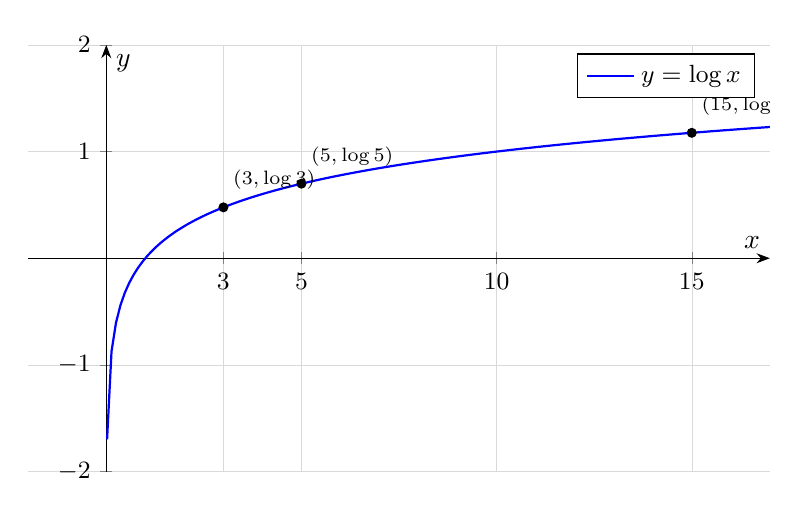
\begin{tikzpicture}
\begin{axis}[
    axis lines = middle,
    xlabel = {$x$}, ylabel = {$y$},
    grid=both,
    grid style={line width=.1pt, draw=gray!30},
    axis line style={-Stealth},
    legend style={font=\small},
    tick label style={font=\small},
    xmin=-2, xmax=17, ymin=-2, ymax=2,
    xtick={0,3,5,10,15},
    ytick={-2,-1,0,1,2},
    width=11cm, height=7cm,
]
\addplot[domain=0.02:17, samples=150, thick, blue] {ln(x)/ln(10)};
\addlegendentry{$y=\log x$}
\addplot[only marks, mark=*, mark size=1.6pt, black] coordinates {(3,0.4771) (5,0.6990) (15,1.1761)};
\node[anchor=south west, font=\scriptsize] at (axis cs:3,0.55) {$(3,\log 3)$};
\node[anchor=south west, font=\scriptsize] at (axis cs:5,0.77) {$(5,\log 5)$};
\node[anchor=south west, font=\scriptsize] at (axis cs:15,1.25) {$(15,\log 15)$};
\end{axis}
\end{tikzpicture}
\end{document}
